
\chapter{Grid Page}
The first page you will be presented with after loading or creating a new project is the Grid Page. This is the main page of MCL and is used to access the firmware's sub-pages and menus.

\begin{center}
	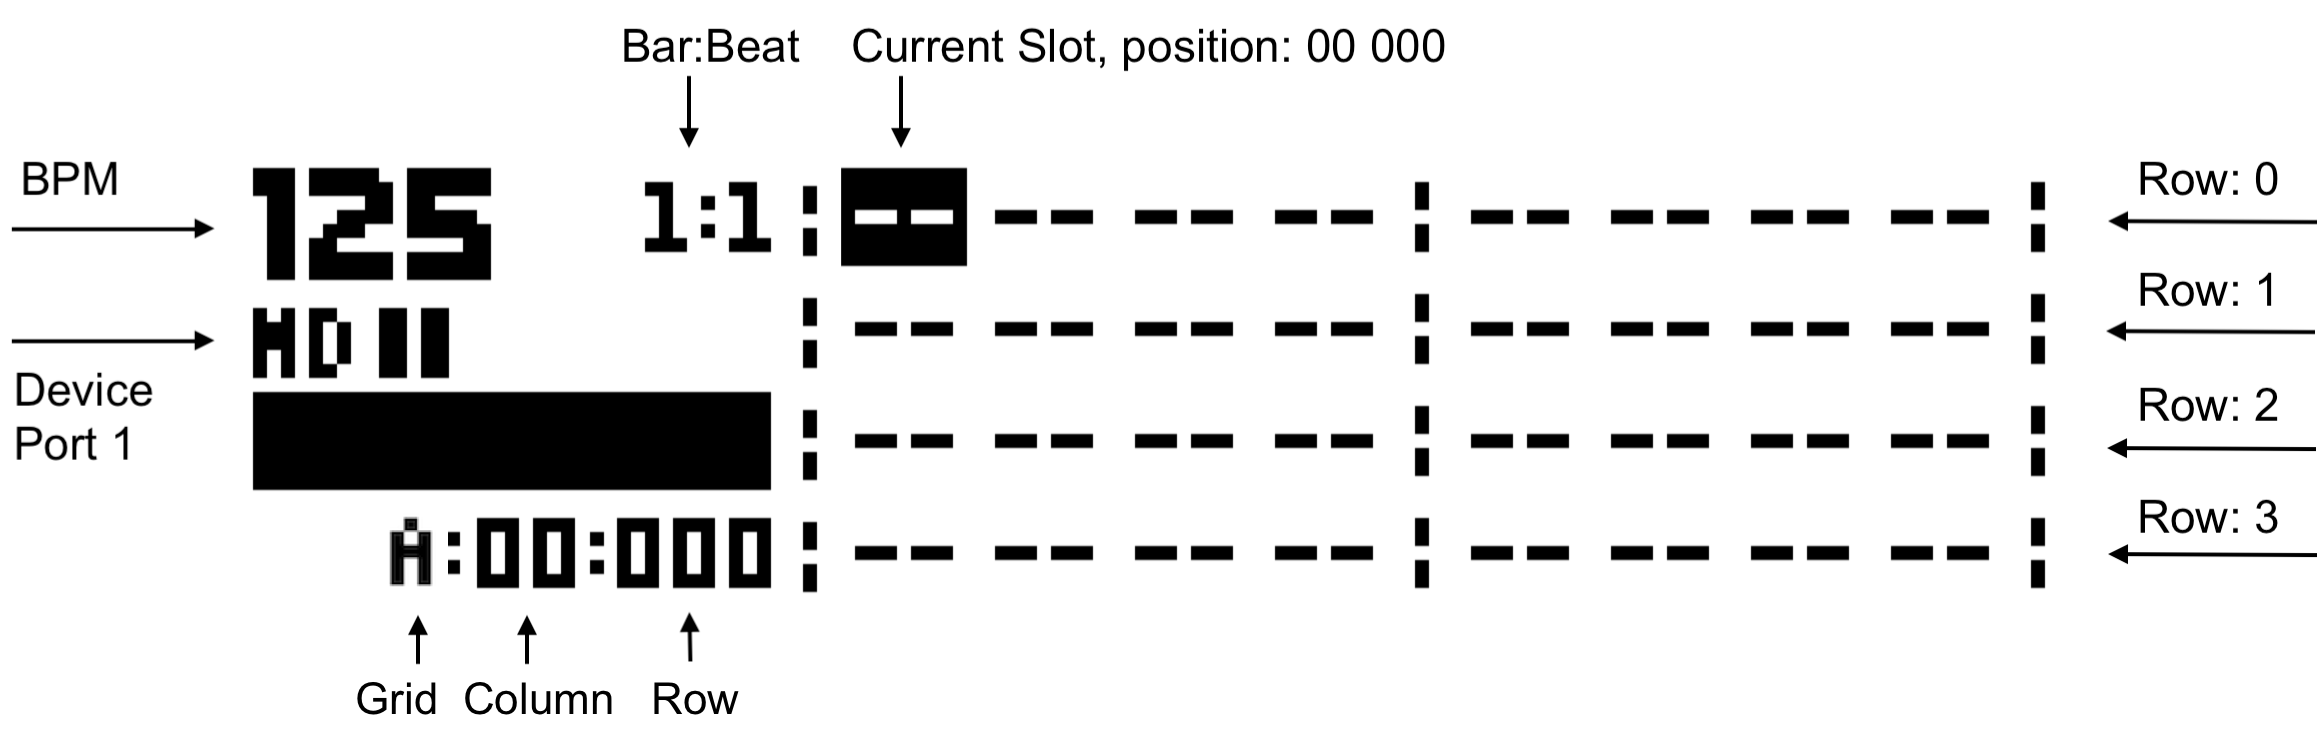
\includegraphics[scale=.40]{grid_init_annot.png}
\end{center}
MCL displays a portion of the active grid on screen. 
Eight slots across four rows are shown.\\
\\
Occupied slots will display the Machine Type associated with the track. For example "BD" for Bass Drum. Unoccupied Slots are represented by two lines of "--" . For clarity, a dashed vertical line is printed after every fourth column.\\\\
An interactive cursor indicates the current slot position and is distinguished by a slot printed with inverted colours. Rotating \textbf{[ Encoder 1 ]} or \textbf{[ Encoder 2 ]} will allow the cursor position to change. When the cursor reaches the edges of the screen you can continue to scroll through the grid.
\\\\
Towards the bottom left corner of the display, the active grid followed by the current slot's column and row are shown.\\\\
The active grid can be toggled between either A or B from the Slot Menu.
\textit{When performing actions such as saving/loading they will apply to the grid that is currently active.}
\\
\encodersbuttons{scrolls the grid horizontally.}{scrolls the grid vertically.}{--}{--}{activates Save page.}{activates PageSelect page.}{activates Load page.}{activates the Slot menu.}